\chapter{Οδηγίες για τη Μορφή της Διατριβής}
\label{ch:Instructions}


\section{Διαδικασία Υποβολής Τελικού Αντίτυπου Διατριβής}
\label{sec:Submission}
Η μορφή αυτή καθιερώθηκε το 2005 και ενημερώθηκε το 2016.\footnote{\url{https://github.com/vvdimako/cseuoi-thesis}.}
Ο φοιτητής θα πρέπει να φέρει τη διατριβή στη μορφή που περιγράφεται, να περάσει την εξέταση, και να κάνει όλες τις απαιτούμενες από τους εξεταστές μετατροπές.
Έπειτα, η διαδικασία που πρέπει να ακολουθήσει είναι η εξής:
\begin{itemize}
	\item Να πάρει την έγκριση του επιβλέποντος για την τελική μορφή της διατριβής (υπογραφή στη φόρμα Δ3).
	\item Να υποβάλλει τη διατριβή στη Σ.Ε.Μ.Σ. για την τελική έγκριση της μορφής (όπως περιγράφεται εδώ) και να προσκομίσει τη φόρμα Δ3 την οποία θα υπογράψει ένα μέλος της επιτροπής.
	\item Να παραδώσει τη διατριβή σε μορφή PDF στο γραφείο Γ17 μαζί με τη φόρμα Δ3.
	\item Να παραλάβει από το γραφείο Γ17 αντίτυπα του εξωφύλλου, τα οποία θα βάλει μπροστά από τη σελίδα τίτλου της διατριβής. H τελευταία σελίδα θα πρέπει να είναι χοντρό λευκό γυαλιστερό χαρτί.
	\item Να παραδώσει τα 3 αντίτυπα για Μεταπτυχιακή Εργασία Εξειδίκευσης ή 5 αντίτυπα για Διδακτορική Διατριβή στο γραφείο Γ17 και να πάρει την υπογεγραμμένη φόρμα Δ3, την οποία θα παραδώσει και στη Γραμματεία μαζί με τα υπόλοιπα έγγραφα για την αποφοίτηση.
\end{itemize}


\section{Διαμόρφωση Κειμένου}
\label{sec:Text}

\subsection{Βασικές Οδηγίες}
\label{subsec:Basic}
Η διατριβή πρέπει να είναι τυπωμένη σε μονή όψη, ενώ το κείμενο πρέπει να είναι εντός των εξής περιθωρίων:
\begin{itemize}
	\item Top: 2.5 cm.
	\item Bottom: 3 cm.
	\item Left: 2.5 cm.
	\item Right: 2.5 cm.
\end{itemize}
Σε όλη τη διατριβή εκτός από τα Σχήματα και τους Πίνακες (συμπεριλαμβανομένων των λεζάντων όμως) πρέπει να χρησιμοποιείται γραμματοσειρά μεγέθους 12 στιγμών.
Οι όροι μπορούν να είναι σε \textit{πλάγια γράμματα}, χρησιμοποιώντας την εντολή \verb|\textit{πλάγια γράμματα}|, συνήθως την πρώτη φορά που χρησιμοποιούνται.
Τα \textbf{έντονα γράμματα} πρέπει να χρησιμοποιούνται μόνο στην περίπτωση που είναι απαραίτητα για την κατανόηση του κειμένου, χρησιμοποιώντας την εντολή \verb|\textbf{έντονα γράμματα}|.

Το κύριο αρχείο είναι το \texttt{SampleThesis.tex}, στο προοίμιο του οποίου θα πρέπει να περάσετε στο πακέτο \texttt{cseuoi-thesis} τις κατάλληλες επιλογές για τη διατριβή σας.
Αν το κείμενο της διατριβής είναι στα Ελληνικά τότε θα πρέπει να περάσετε την επιλογή \texttt{gr}, ενώ αν το κείμενο της διατριβής είναι στα Αγγλικά τότε θα πρέπει να περάσετε την επιλογή \texttt{en}.
Για τη στοιχειοθεσία Μεταπτυχιακής Εργασίας Εξειδίκευσης θα πρέπει να περάσετε την επιλογή \texttt{msc}, ενώ για τη στοιχειοθεσία Διδακτορικής Διατριβής θα πρέπει να περάσετε την επιλογή \texttt{phd}.
Στην περίπτωση της Μεταπτυχιακής Εργασίας Εξειδίκευσης θα πρέπει επιπλέον να περάσετε την κατάλληλη επιλογή για μία από τις εξής εξειδικεύσεις:
\begin{itemize}
	\item Υπολογιστικά Συστήματα: \texttt{systems}.
	\item Θεωρία Επιστήμης Υπολογιστών: \texttt{theory}.
	\item Λογισμικό: \texttt{software}.
	\item Επιστημονικοί Υπολογισμοί: \texttt{scicomp}.
	\item Τεχνολογίες - Εφαρμογές: \texttt{techapps}.
\end{itemize}
Στην περίπτωση της Διδακτορικής Διατριβής δεν περνάτε επιλογή για εξειδίκευση.

Στη συνέχεια του ίδιου αρχείου θα πρέπει να συμπληρώσετε τα στοιχεία σας στις αντίστοιχες εντολές, αφαιρώντας την εντολή \verb|\colorbox{gray}{}|.
Ειδικότερα, τα στοιχεία που θα πρέπει να συμπληρώσετε είναι ο τίτλος της διατριβής, το ονοματεπώνυμο του φοιτητή, ο μήνας και το έτος αποφοίτησης, καθώς και το ονοματεπώνυμο και τη βαθμίδα του επιβλέπων καθηγητή.
Τα παραπάνω στοιχεία θα πρέπει να τα συμπληρώσετε και στα Ελληνικά και στα Αγγλικά προκειμένου να χρησιμοποιηθούν κατάλληλα σε διάφορα σημεία της διατριβής, όπως η σελίδα τίτλου και οι σελίδες με τις περιλήψεις.
Αν κάποια τμήματα της διατριβής σας είναι σκιασμένα, είτε δεν έχετε συμπληρώσει τα αντίστοιχα στοιχεία σας είτε δεν αφαιρέσατε την εντολή \verb|\colorbox{gray}{}| όταν τα συμπληρώσατε.

\subsection{Κεφάλαια}
\label{subsec:Chapters}
Για να ορίσετε τον τίτλο ενός κεφαλαίου, πρέπει να χρησιμοποιήσετε την εντολή \verb|\chapter{Τίτλος Κεφαλαίου}|.
Παρόμοια, για τους τίτλους ενοτήτων χρησιμοποιείτε την εντολή \verb|\section{Τίτλος Ενότητας}|, ενώ για τίτλους υποενοτήτων την εντολή \verb|\subsection{Τίτλος Υποενότητας}|.
Είναι επιθυμητό να εισάγετε και μία ετικέτα κάθε φορά που χρησιμοποιείτε τις παραπάνω εντολές, το οποίο γίνεται με την εντολή \verb|\label{Ετικέτα}|, προκειμένου να μπορείτε να αναφέρεστε στο αντίστοιχο σημείο του κειμένου με την εντολή \verb|\ref{Ετικέτα}|.

To πακέτο \texttt{xgreek}\footnote{\url{https://www.ctan.org/pkg/xgreek?lang=en}.} ορίζει διάφορες χρήσιμες μακροεντολές, οι οποίες επιτρέπουν την εύκολη χρήση χαρακτήρων που είναι δύσκολα προσβάσιμοι από το πληκτρολόγιο.
Μερικές από αυτές τις μακροεντολές είναι οι εξής:
\begin{itemize}
	\item Άνω τόνος (\anwtonos): \verb|\anwtonos|.
	\item Άνω τελεία (\anoteleia): \verb|\anoteleia|.
	\item Σύμβολο του Ευρώ (\euro): \verb|\euro|.
	\item Σύμβολο τοις χιλίοις (\permill): \verb|\permill|.
\end{itemize}

Όταν θεωρείτε ότι είναι απολύτως απαραίτητο, μπορείτε να εισάγετε μία υποσημείωση με την εντολή \verb|\footnote{Αυτή είναι μία υποσημείωση.}|, η οποία εμφανίζεται στο κάτω μέρος της αντίστοιχης σελίδας\footnote{Αυτή είναι μία υποσημείωση.}.
Αν θέλετε να εισάγετε έναν νέο όρο στο ευρετήριο, θα πρέπει να χρησιμοποιήσετε την εντολή\index{νέος όρος} \verb|\index{νέος όρος}|.
Για κάθε υποόρο που θέλετε να προστεθεί σε έναν προηγούμενο όρο, θα πρέπει να χρησιμοποιήσετε την εντολή\index{νέος όρος!υποόρος} \verb|\index{νέος όρος!υποόρος}|.

\subsection{Παραρτήματα}
\label{subsec:Appendices}
Προαιρετικά, μπορείτε να εισάγετε ένα ή περισσότερα παραρτήματα, τα οποία θα βρίσκονται μετά τη βιβλιογραφία και πριν το ευρετήριο.
Σε αντίθεση με τα κεφάλαια της διατριβής, η αρίθμηση των παραρτημάτων γίνεται με κεφαλαίους χαρακτήρες.


\section{Σχήματα}
\label{sec:Figures}
Τα σχήματα και οι λεζάντες τους πρέπει να είναι πάντα κεντραρισμένα και εντός των περιθωρίων του κειμένου.
Για να εισάγουμε ένα σχήμα στο κείμενο, χρησιμοποιούμε τις παρακάτω εντολές:

\begin{verbatim}
\begin{figure}[t]
 \centering
 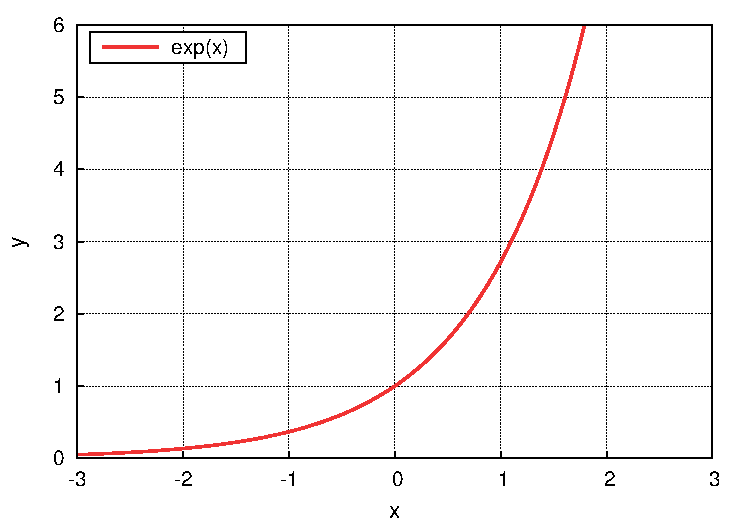
\includegraphics[width=0.65\textwidth]{Figures/ExponentialFunction.pdf}
 \caption{Η εκθετική συνάρτηση.}
 \label{fig:ExponentialFunction}
\end{figure}
\end{verbatim}

\begin{figure}[t]
	\centering
	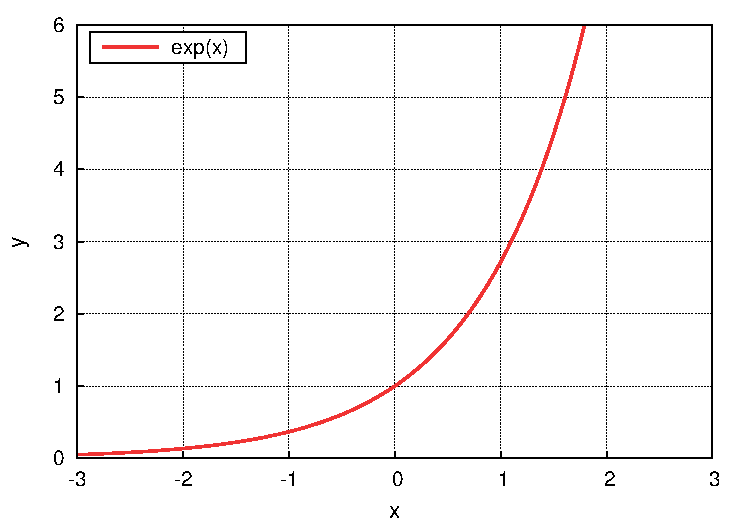
\includegraphics[width=0.65\textwidth]{Figures/ExponentialFunction.pdf}
	\caption{Η εκθετική συνάρτηση.}
	\label{fig:ExponentialFunction}
\end{figure}

Το αποτέλεσμα των παραπάνω εντολών φαίνεται στο Σχήμα~\ref{fig:ExponentialFunction}, ενώ σε περίπτωση που θέλουμε να αναφερθούμε σε αυτό μέσα στο κείμενο, χρησιμοποιούμε την εντολή \verb|Σχήμα~\ref{fig:ExponentialFunction}|.
Αν θέλουμε να εισάγουμε σε ένα σχήμα πολλές εικόνες μαζί, τότε χρησιμοποιούμε τις παρακάτω εντολές:

\begin{verbatim}
\begin{figure}[t]
 \centering
 \begin{subfigure}[t]{0.3\textwidth}
  \centering
  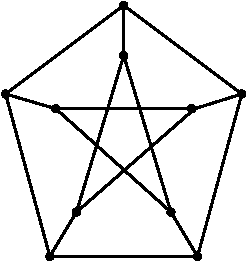
\includegraphics[height=0.15\textheight]{Figures/GraphA.pdf}
  \caption{}
  \label{subfig:GraphA}
 \end{subfigure}
 \hfill
 \begin{subfigure}[t]{0.3\textwidth}
  \centering
  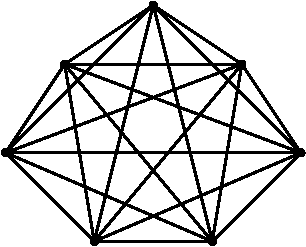
\includegraphics[height=0.15\textheight]{Figures/GraphB.pdf}
  \caption{}
  \label{subfig:GraphB}
 \end{subfigure}
 \hfill
 \begin{subfigure}[t]{0.3\textwidth}
  \centering
  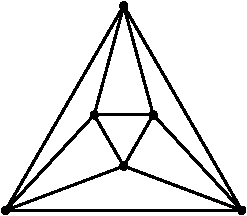
\includegraphics[height=0.15\textheight]{Figures/GraphC.pdf}
  \caption{}
  \label{subfig:GraphC}
 \end{subfigure}
 \caption{Τρία γραφήματα.}
 \label{fig:ThreeGraphs}
\end{figure}
\end{verbatim}

\begin{figure}[t]
	\centering
	\begin{subfigure}[t]{0.3\textwidth}
		\centering
		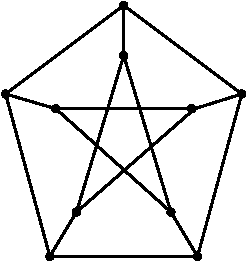
\includegraphics[height=0.15\textheight]{Figures/GraphA.pdf}
		\caption{}
		\label{subfig:GraphA}
	\end{subfigure}
	\hfill
	\begin{subfigure}[t]{0.3\textwidth}
		\centering
		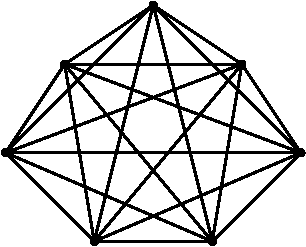
\includegraphics[height=0.15\textheight]{Figures/GraphB.pdf}
		\caption{}
		\label{subfig:GraphB}
	\end{subfigure}
	\hfill
	\begin{subfigure}[t]{0.3\textwidth}
		\centering
		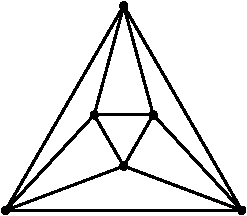
\includegraphics[height=0.15\textheight]{Figures/GraphC.pdf}
		\caption{}
		\label{subfig:GraphC}
	\end{subfigure}
	\caption{Τρία γραφήματα.}
	\label{fig:ThreeGraphs}
\end{figure}

Με τις παραπάνω εντολές εισάγαμε στο Σχήμα~\ref{fig:ThreeGraphs} τρία υποσχήματα, στα οποία μπορούμε να αναφερθούμε και ξεχωριστά αν θέλουμε, χρησιμοποιώντας τις αντίστοιχες ετικέτες που τους αναθέσαμε.


\section{Πίνακες}
\label{sec:Tables}
Με παρόμοιες εντολές μπορούμε να εισάγουμε και πίνακες.
Για παράδειγμα, με τις παρακάτω εντολές δημιουργούμε τον Πίνακα~\ref{tab:Example}.

\begin{verbatim}
\begin{table}[t]
 \centering
 \caption{Ένας Πίνακας.}
 \label{tab:Example}
 \begin{tabular}{| l || l | l | l |}
  \hline
  κελί 1 & κελί 2 & κελί 3 & κελί 4\\
  \hline
  \hline
  κελί 5 & κελί 6 & κελί 7 & κελί 8\\
  \hline
  κελί 9 & κελί 10 & κελί 11 & κελί 12\\
  \hline
  κελί 13 & κελί 14 & κελί 15 & κελί 16\\
  \hline
  κελί 17 & κελί 18 & κελί 19 & κελί 20\\
  \hline
 \end{tabular}
\end{table}
\end{verbatim}

\begin{table}[t]
	\centering
	\caption{Ένας Πίνακας.}
	\label{tab:Example}
	\begin{tabular}{| l || l | l | l |}
		\hline
		κελί 1 & κελί 2 & κελί 3 & κελί 4\\
		\hline
		\hline
		κελί 5 & κελί 6 & κελί 7 & κελί 8\\
		\hline
		κελί 9 & κελί 10 & κελί 11 & κελί 12\\
		\hline
		κελί 13 & κελί 14 & κελί 15 & κελί 16\\
		\hline
		κελί 17 & κελί 18 & κελί 19 & κελί 20\\
		\hline
	\end{tabular}
\end{table}


\section{Αλγόριθμοι}
\label{sec:Algorithms}
Για τη στοιχειοθεσία αλγορίθμων σε μορφή ψευδοκώδικα, όπως φαίνεται στον Αλγόριθμο~\ref{alg:Example} για παράδειγμα, χρησιμοποιούμε τις παρακάτω εντολές:

\begin{verbatim}
\begin{algorithm}[t]
 \caption{Υπολογισμός $y = x^n$.}
 \label{alg:Example}
 \begin{algorithmic}[1]
  \REQUIRE $n \geq 0 \vee x \neq 0$
  \ENSURE $y = x^n$
  \STATE $y \leftarrow 1$
  \IF{$n < 0$}
  \STATE $X \leftarrow 1 / x$
  \STATE $N \leftarrow -n$
  \ELSE
  \STATE $X \leftarrow x$
  \STATE $N \leftarrow n$
  \ENDIF
  \WHILE{$N \neq 0$}
  \IF{$N$ is even}
  \STATE $X \leftarrow X \times X$
  \STATE $N \leftarrow N / 2$
  \ELSE[$N$ is odd]
  \STATE $y \leftarrow y \times X$
  \STATE $N \leftarrow N - 1$
  \ENDIF
  \ENDWHILE
 \end{algorithmic}
\end{algorithm}
\end{verbatim}

\begin{algorithm}[t]
	\caption{Υπολογισμός $y = x^n$.}
	\label{alg:Example}
	\begin{algorithmic}[1]
		\REQUIRE $n \geq 0 \vee x \neq 0$
		\ENSURE $y = x^n$
		\STATE $y \leftarrow 1$
		\IF{$n < 0$}
		\STATE $X \leftarrow 1 / x$
		\STATE $N \leftarrow -n$
		\ELSE
		\STATE $X \leftarrow x$
		\STATE $N \leftarrow n$
		\ENDIF
		\WHILE{$N \neq 0$}
		\IF{$N$ is even}
		\STATE $X \leftarrow X \times X$
		\STATE $N \leftarrow N / 2$
		\ELSE[$N$ is odd]
		\STATE $y \leftarrow y \times X$
		\STATE $N \leftarrow N - 1$
		\ENDIF
		\ENDWHILE
	\end{algorithmic}
\end{algorithm}


\section{Μαθηματικά}
\label{sec:Mathematics}
Για τη στοιχειοθεσία μαθηματικών εκφράσεων χρησιμοποιούμε με παρόμοιο τρόπο τα παρακάτω περιβάλλοντα:
\begin{itemize}
	\item Εξίσωση: \verb|\begin{equation} ... \end{equation}|.

	\begin{equation}
		S_{n} = 1 + \sum_{k=1}^{n}\frac{1}{k^{2} + k}\,,\quad n \in \mathbb{N}\,.
		\label{eq:Example}
	\end{equation}

	\item Θεώρημα: \verb|\begin{theorem} ... \end{theorem}|.

	\begin{theorem}
		Τhe square of the hypotenuse (the side opposite the right angle) is equal to the sum of the squares of the other two sides.
	\end{theorem}

	\item Λήμμα: \verb|\begin{lemma} ... \end{lemma}|.

	\begin{lemma}
		If a prime divides the product of two numbers, it must divide at least one of those numbers.
	\end{lemma}

	\item Πόρισμα: \verb|\begin{corollary} ... \end{corollary}|.

	\begin{corollary}
		In any right triangle, the hypotenuse is greater than any one of the other sides, but less than their sum.
	\end{corollary}

	\item Γεγονός: \verb|\begin{fact} ... \end{fact}|.

	\begin{fact}
		It takes 8 minutes 17 seconds for light to travel from the Sun’s surface to the Earth.
	\end{fact}

	\item Σημείωση: \verb|\begin{remark} ... \end{remark}|.

	\begin{remark}
		This is a remark.
	\end{remark}

	\item Ορισμός: \verb|\begin{definition} ... \end{definition}|.

	\begin{definition}
		Addition is bringing two or more numbers (or things) together to make a new total.
	\end{definition}

	\item Παρατήρηση: \verb|\begin{observation} ... \end{observation}|.

	\begin{observation}
		This is an observation.
	\end{observation}

	\item Aπόδειξη: \verb|\begin{proof} ... \end{proof}|.

	\begin{theorem}[Fermat's Last Theorem]
		There are no positive integers $x$, $y$, and $z$ that satisfy the equation $x^{n} + y^{n} = z^{n}$ for any integer value of $n > 2$.
	\end{theorem}
	\begin{proof}
		``I have discovered a truly marvellous proof of this, which this margin is too narrow to contain.''
	\end{proof}
\end{itemize}


\section{Διαχείριση Βιβλιογραφίας}
\label{sec:Bibliography}
Για τη δημιουργία της βιβλιογραφίας χρησιμοποιούμε το πακέτο BibTeX.
Για αυτό απαιτείται μία βιβλιογραφική βάση δεδομένων, η οποία αποθηκεύεται ως ένα απλό αρχείο κειμένου με κατάληξη bib.
Το αρχείο αυτό περιέχει καταχωρήσεις της παρακάτω μορφής:

\begin{verbatim}
@article{Newman2003a,
 author = {Newman, Mark E. J.},
 title = {The Structure and Function of Complex Networks},
 journal = {SIAM Review},
 volume = {45},
 number = {2},
 pages = {167--256},
 year = {2003},
 doi = {10.1137/S003614450342480}
}
\end{verbatim}

Κάθε καταχώρηση ξεκινά με τη δήλωση του τύπου της αναφοράς.
Το παραπάνω παράδειγμα αποτελεί αναφορά σε ένα άρθρο περιοδικού, επομένως η καταχώρηση ξεκινά με τη δήλωση \verb|@article|.
Στη συνέχεια αναθέτουμε ένα μοναδικό κλειδί στην καταχώρηση, π.χ. \verb|Newman2003a|, το οποίο χρησιμοποιούμε στο κείμενο της διατριβής για να αναφερθούμε σε αυτή με την εντολή \verb|\cite{Newman2003a}|.
Τέλος, συμπληρώνουμε τα πεδία του αντίστοιχου τύπου αναφοράς, μερικά από τα οποία είναι υποχρεωτικά.
Για παράδειγμα, στις καταχωρήσεις άρθρων είναι υποχρεωτική η συμπλήρωση των πεδίων \verb|author|, \verb|title|, \verb|journal|, και \verb|year|.

Η βιβλιογραφία της διατριβής στοιχειοθετείται αυτόματα μετά το τέλος των κεφαλαίων, με κάθε καταχώρηση να έχει έναν χαρακτηριστικό αριθμό.
Ο χαρακτηριστικός αριθμός της κάθε καταχώρησης εμφανίζεται μεταξύ αγκυλών στα σημεία του κειμένου της διατριβής όπου αναφερθήκαμε σε αυτή την καταχώρηση.
Για παράδειγμα, σε αυτήν την πρόταση αναφερόμαστε σε ένα άρθρο περιοδικού~\cite{Newman2003a}, σε μία εργασία συνεδρίου~\cite{DeCandia2007a}, σε μία τεχνική αναφορά~\cite{Jain1984a}, και σε ένα βιβλίο~\cite{Golumbic2004a}.